\documentclass[paper=a4,fontsize=12pt]{scrartcl}
\usepackage{geometry}
\usepackage{graphicx}
\usepackage{wrapfig}
\usepackage{titling}
\usepackage{float}
\usepackage[format=plain]{caption}
\geometry{verbose, a4paper, tmargin=25mm, bmargin=25mm, lmargin=25mm, rmargin=25mm}

\usepackage[utf8]{inputenc}
\usepackage[ngerman]{babel}
\usepackage{fancyhdr} %Paket laden
\pagestyle{fancy} %eigener Seitenstil
\fancyhf{} %alle Kopf- und Fußzeilenfelder bereinigen
\fancyhead[L]{
\includegraphics[width=3cm]{img/logo_bfh_de.jpg}} %Kopfzeile links
\fancyhead[C]{} %zentrierte Kopfzeile
\fancyhead[R]{Janosch Rohdewald, Marco Füllemann} %Kopfzeile rechts
\renewcommand{\headrulewidth}{0.4pt} %obere Trennlinie
\fancyfoot[C]{\thepage} %Seitennummer
\renewcommand{\footrulewidth}{0.4pt} %untere Trennlinie


\title{Wo ist Walter}
\author{Marco Füllemann\newline Janosch Rohdewald}
\date{3. Dezember 2014}

\begin{document}
\pagestyle{empty}
\hbox{ % Horizontal box
  \hspace*{0.2\textwidth} % Whitespace to the left of the title page
  \rule{1pt}{\textheight} % Vertical line
  \hspace*{0.05\textwidth} % Whitespace between the vertical line and title page text
  \parbox[b]{0.75\textwidth}{ % Paragraph box which restricts text to less than the width of the page

  {\noindent\Huge\bfseries \thetitle}\\[2\baselineskip] % Title
  {\large \textit{Suche mit Hilfe von Bild-Operatoren in Matlab}}\\[4\baselineskip] % Tagline or further description
  {\Large \textsc{\theauthor}} % Author name
  \vspace{0.5\textheight} % Whitespace between the title block and the publisher
  }}
\newpage
\pagestyle{fancy}
\section*{Zusammenfassung}
\section*{Einleitung}
\section*{Grundlagen}
\subsection*{Farbkanal Extraktion}
\subsection*{Morphologische Operatoren}
\subsection*{Hough Transformation}
\newpage
\section*{Vorgehen, Methoden, Analysen}
Wir haben unser Vorgehen auf den bereits erlernten Grundlagen in der CPVR-Vertiefung des Studiums aufgebaut. Dabei wollten wir die Aufgabe nicht mit Hilfe einer Ähnlichkeitssuche von Walters Bild lösen. Wir haben uns entschieden wichtige Merkmale von Walter durch die Anwendung von lokalen und globalen Operatoren zu finden. Dabei ist wichtig zu erwähnen, dass es dadurch nicht möglich ist Walter anhand eines einzigen Merkmals zu finden. Deshalb wurde der Ansatz gewählt die Brille durch eine Kreis-Hough Transformation zu finden und das T-Shirt durch das horizontale rot-weiss Muster.
\subsection*{Brille}
Um eine einfachere Entwicklung des Algorithmus zu ermöglichen, wurde mit einem Ausschnitt des Bildes gearbeitet, welcher wie folgt gewählt wurde:

\begin{figure}[htbp]
\centering
\begin{minipage}{.5\textwidth}
  \centering
  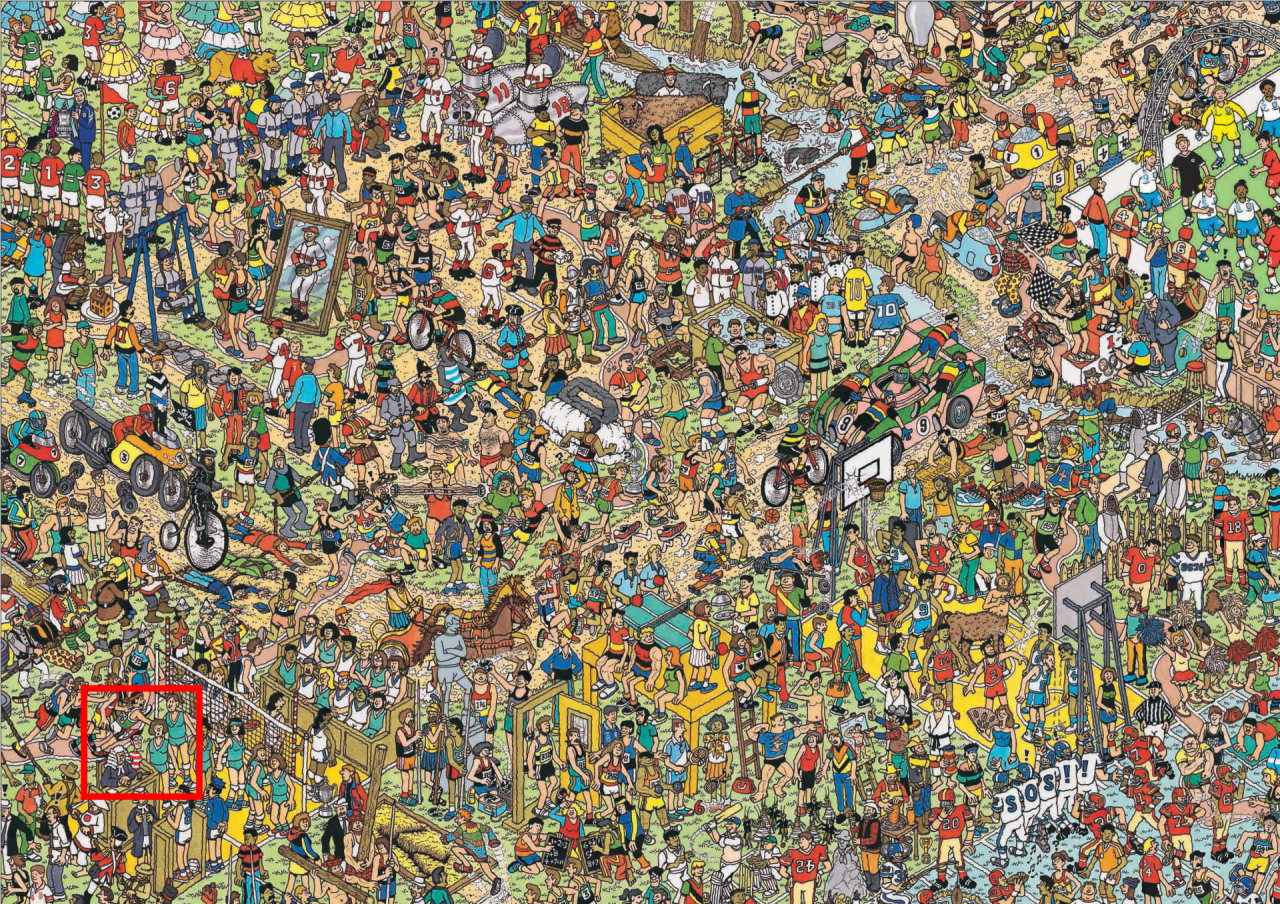
\includegraphics[height=.6\linewidth]{img/WallyWembleyGlassesSelection.png}
  \caption{Wembley Stadion}
\end{minipage}%
\begin{minipage}{.5\textwidth}
  \centering
  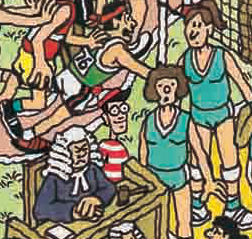
\includegraphics[height=.6\linewidth]{img/WallyWembleyCroppedGlasses.png}
  \caption{Ausschnitt Brillendetektion}
\end{minipage}
\end{figure}
\subsubsection*{Brillenrand} 
Die erste Idee war die Brille durch eine Extraktion der Brillenränder zu finden.\\

\noindent\begin{minipage}[t]{0.6\textwidth}
Dafür wurden zuerst die (schwarzen) Pixel, bei welchen alle 3 RGB Kanäle Werte kleiner als 0.3 (Hex 0x4C) sind, extrahiert.  
\end{minipage}
\hfill
\begin{minipage}[c]{0.4\textwidth}
  \flushright
  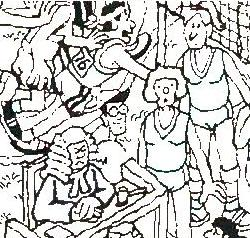
\includegraphics[width=0.7\textwidth]{img/glasses_blackExtract.jpg}
\end{minipage}



\begin{wrapfigure}{R}{5.5cm}
\caption{A wrapped figure}\label{wrap-fig:1}

\end{wrapfigure} 


%\begin{SCfigure}
%  \centering
%  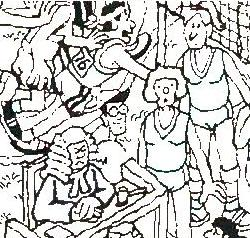
\includegraphics[height=.4\linewidth]{img/glasses_blackExtract.jpg}
%  \caption{}
%\end{SCfigure}
%\begin{SCfigure}
%  \centering
%  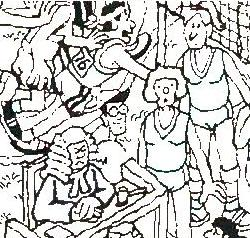
\includegraphics[height=.4\linewidth]{img/glasses_blackExtract.jpg}
%  \caption{Um die Ränder der Brille zu schliessen wurde ein binäres Closing angewandt.}
%\end{SCfigure}
\newpage
\subsection*{T-Shirt}
\section*{Ergebnisse, Resultate}

\end{document}
